\documentclass[10pt,twocolumn]{witseiepaper}

%
% All KJN's macros and goodies (some shameless borrowing from SPL)
\usepackage{KJN}
\usepackage{subcaption}
\usepackage{listings}
\usepackage{amsmath}
\usepackage{epstopdf}
\usepackage{xcolor}
\usepackage{textcomp}
\usepackage{listings}
\usepackage{alltt}
\usepackage{matlab-prettifier}
\usepackage{graphicx}
\usepackage{changes}
\usepackage{makecell}
\usepackage{verbatim}
\usepackage{algorithm,algpseudocode}
\usepackage{balance}
\usepackage{pdfpages}
\usepackage{tikz} % for drawing stuff
\usetikzlibrary{positioning} % for relative coordinates
\usepackage{color} %red, green, blue, yellow, cyan, magenta, black, white
\definecolor{mygreen}{RGB}{28,172,0} % color values Red, Green, Blue
\definecolor{mylilas}{RGB}{170,55,241}
%\usepackage{flafter}

\lstset{language=Matlab, % Set colour for matlab code
	breaklines=true,%
	morekeywords={matlab2tikz},
	keywordstyle=\color{blue},%
	morekeywords=[2]{1}, keywordstyle=[2]{\color{black}},
	identifierstyle=\color{black},%
	stringstyle=\color{mylilas},
	commentstyle=\color{mygreen},%
	showstringspaces=false,%without this there will be a symbol in the places where there is a space
	numbers=left,%
	numberstyle={\tiny \color{black}},% size of the numbers
	numbersep=9pt, % this defines how far the numbers are from the text
	emph=[1]{for,end,break},emphstyle=[1]\color{red}, %some words to emphasise
	%emph=[2]{word1,word2}, emphstyle=[2]{style},    
}
\usepackage{lmodern}
\newcommand*{\escape}[1]{\texttt{\textbackslash#1}}

%
% PDF Info
%
\ifpdf
\pdfinfo{
/Title (FILE TRANSFER APPLICATION)
/Author (KJ Butkow, Jared Ping)
/CreationDate (D:201803151731)
/ModDate (D:200510121530)
/Subject (FILE TRANSFER APPLICATION)
/Keywords ()
}
\fi

%%%%%%%%%%%%%%%%%%%%%%%%%%%%%%%%%%%%%%%%%%%%%%%%%%%%%%%%%%%%%%%%%%%%%%%%%%%%%%%
\begin{document}


\title{FILE TRANSFER APPLICATION  \\ ELEN4017 Project Report}

\author{Kayla-Jade Butkow (714227) and Jared Ping (704447)
\thanks{School of Electrical \& Information Engineering, University of the
Witwatersrand, Private Bag 3, 2050, Johannesburg, South Africa}
}


%%%%%%%%%%%%%%%%%%%%%%%%%%%%%%%%%%%%%%%%%%%%%%%%%%%%%%%%%%%%%%%%%%%%%%%%%%%%%%%
%
\abstract{}

\keywords{client, file transfer protocol, server}

\maketitle
\thispagestyle{empty}
\pagestyle{plain}
\setcounter{page}{1}

%%%%%%%%%%%%%%%%%%%%%%%%%%%%%%%%%%%%%%%%%%%%%%%%%%%%%%%%%%%%%%%%%%%%%%%%%%%%%%%
%
\section{INTRODUCTION}
The File Transfer Protocol (FTP) is essential in the implementation of a File Transfer Application. The File Transfer Protocol allows for the transfer of files between two end systems \cite{kurose}. The FTP protocol runs on top of TCP and, uniquely, makes use of two TCP connections: a control connection and a data connection \cite{kurose}. The data connection is non-persistent, and is created when the transfer of data is required \cite{kurose}. A File Transfer Application consists of an FTP server and an FTP client. This report presents the design, implementation and testing of a File Transfer Application, including an overview of the system, details of the implemented code, results and a critical analysis of the system. The division of labour between group members is also discussed.

\section{SYSTEM OVERVIEW}
\subsection{FTP Server}
The FTP server runs from the user's local host and allows users to connect through a locally hosted FTP client, as well as through clients on the same network. The server facilitates the storage of files and a user management system. The server is capable of running on any Unix based system.

The server's user management system functions by requesting users to authenticate themselves upon connecting to the server. This information is used to provide each user with their own maintained file repository. The repository implementation allows the user to only access their files and prevents users from being aware of other user repositories, providing a secure and user-tailored experience. Unauthenticated users will be unable to perform any modification operations such as uploading and deleting files.

The server has been created in accordance with the RFC 959 standards to allow for compatibility with standard FTP clients, allowing users to connect to the server from a range of clients. An extensive number of RFC commands have been implemented to provide improved compatibility and functionality for FTP clients which utilise the additional commands. A server logger has also been implemented to track client requests in real-time for server monitoring and debugging capabilities.

Multi-threading has been utilised in the development of the server to facilitate simultaneous client connections. This supports both connection and server request operations, allowing for multiple users to connect, browse directories, and upload and download files concurrently.

\subsubsection*{Unimplemented Features:}
The file structure type of the server is defaulted to the file structure, with the page and record structures not being implemented due to complexity and time overhead. The data transmission mode of the server is defaulted to the stream mode, with the block and compression modes not being implemented due to complexity and time overhead. The default structure type and data transmission mode is set to be the file structure and stream mode respectively for any FTP application in accordance with RFC 959, thus no client compatibility issues will be encountered \cite{rfc}. The lack of compression data transmission mode results in a lower available bandwidth for very large network transmissions \cite{rfc}.

\subsection{FTP Client}
The FTP client runs from the user's local host and allows the user to interact with the FTP server in order to transfer files. In order to improve user experience, a client with a graphical user interface (GUI) was implemented. 

The client allows the user to specify the FTP server address that they wish to connect to, as well as the port that the server is running on. The user is also able to input their username and password for the FTP server they are connecting to.

Once the user has successfully connected to the FTP server, they are able to view their local file system as well as the remote file system within the client GUI. The user is also able to navigate both file systems. Once the required file is found, the user is able to upload the file to the remote server from the local file system, or download the file from the remote system to the local storage. When uploading a file, the file is saved to the currently selected directory on the server. If a directory has not been selected by the user, the file is saved to the home directory of the user's remote repository. Likewise, when the user is downloading a file, the file is saved to the current local folder, or if none is selected, to the user's home directory. On Mac OS X operating systems, this home directory is found at \textit{/Users/Username}. If a file is selected rather than a directory, the downloaded file is saved in the directory in which the selected file is found.

The user also has the ability to delete files or folders, as well as to recursively remove a folder and all of its contents. Finally, the user is able to create a folder on the server in the base directory of their choosing. If a file is selected rather than a base directory, the new directory is saved in the directory containing the selected file.

Once the client has finished using the FTP connection, they can disconnect from the server and connect to another server if they wish to.

\subsubsection*{Unimplemented Features:}
The feature to change the file structure from file to record or page was not implemented. This was not implemented since the implementation was complex and deemed unnecessary since any file can be transfered using the file structure. Furthermore, since the file structure is the default type, any server that the client wishes to interact with will be compatible with the file structure type \cite{rfc}. The client also does not allow the user the opportunity to change the transmission mode from stream to block or compression. Once again, since stream mode is the default mode, any FTP server must accept stream mode, meaning that implementation of the other types in unnecessary \cite{rfc}. The client also does not have implementation to allow the user to append data onto the end of an existing text file.

** Rename from and to if not implemented

\section{COMMANDS AND REPLY CODES} \label{sec:commands}

\section{IMPLEMENTATION DETAILS}
The server and the client were both implemented using Python 3. On both systems, all communication sockets are created using the Python \texttt{socket} module \cite{socket}. The sending and receiving of messages are also performed using methods from this module. Interfacing with the operating system is performed using the \texttt{os} module \cite{os}. This module allows for the traversing of paths in the operating system, as well as for saving and opening files \cite{os}. 

Communication between the server and client is performed through the establishment of a TCP connection. This TCP connection acts as a control connection to transfer FTP commands and replies between the client and the server \cite{kurose}. When sending FTP commands to the server, the messages are formatted using the format in \figref{fig:commandformat}. In the figure, SP indicates a space and CRLF is the end of line sequence (\escape{r}\escape{n}). All communicated commands utilise \texttt{UTF-8} encoding to ensure communication compatibility.

\begin{figure}[h]
	\centering
	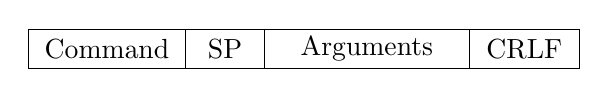
\begin{tikzpicture}
	\draw 
	(0,0) rectangle (2,-0.5) node[pos=.5] {Command}
	(2,0) rectangle (3, -0.5) node[pos=.5] {SP}
	(3,0) rectangle (5.6,-0.5) node[pos=.5] {Arguments}
	(5.6, 0) rectangle (7,-0.5) node[pos=.5] {CRLF}
	;
	\end{tikzpicture}
	\caption{FTP Command Format}
	\label{fig:commandformat}
\end{figure}

\subsection{Server}
In order to host client connections the server listens for any incoming connections which is established as a TCP connection between the two endpoints. A \texttt{serverListener()} function was created for this purpose with a socket configured to utilise the \texttt{SO\_REUSEADDR} argument which allows for active client connections to be maintained in the event of a sudden server restart. 

Each new incoming client connection was handled by binding the connection to a new thread to handle simultaneous connections. The instantiated thread waits for client transmission using the \texttt{recv()} function which is then decoded and the requested command is executed with a resulting response code that is encoding and sent back to the client using the \texttt{send()} function. The server utilises responses to provide the client with a result corresponding to the requested command. The aforementioned process is illustrated in \figref{fig:server}. These responses indicate command successes, errors, mode changes, and other relevant indicators. These response codes are described in Section~\ref{sec:commands}

\subsubsection*{Configuration:}
The server provides a range of configuration commands for clients to utilise based on how they are attempting to interact with the server. \texttt{PASV} specifies the server Data Transfer Process (DTP) to listen on a non-default data port to wait for a connection rather than initiate one upon receipt of a transfer command. \texttt{PORT} offers similar functionality however, the port is explicitly specified by the client. \texttt{MODE} specifies the data transfer method to be utilised by the server. \texttt{STRU} specifies the type of file structure to be used for representation of data by the server.

\subsubsection*{File browser:}
The server provides a range of file browser commands that offer the functionality of file browser commands in a terminal client. \texttt{PWD} prints the path of the current working directory. \texttt{CWD} allows for the client to change their current working directory path to another location. \texttt{CDUP} allows for the client to change the current working directory to the parent directory. \texttt{MKD} allows the client to make a directory in the current directory. \texttt{RMD} allows the client to remove the specified directory from the current directory. \texttt{DELE} allows the client to remove the specified directory from the current directory. \texttt{LIST} provides a list of content contained within the current working directory. Any deletion operation requires a user to be authenticated. A custom utility was created for \texttt{LIST} function to provide the client with as comprehensive information of the directory contents such as file permissions, file size and user group. \texttt{RNFR} and \texttt{RNTO} allows a client to rename a folder or file on the server.

\subsubsection*{File transfer:}
The server provides comprehensive functionality in its ability to handle file uploads and downloads. This begins with allowing clients to specify the file type through the \texttt{TYPE} command, allowing the differentiation between ASCII and binary file transfer. \texttt{RETR} and \texttt{STOR} facilitate a file being downloaded and uploaded respectively from the server. Furthermore, \texttt{APPE} allows a file to be uploaded with its content being appended to the file if it already exists on the server otherwise it server the same purpose as \texttt{STOR}. Any upload operation requires a user to be authenticated.

\subsubsection*{Miscellaneous:}
In addition to the existing server infrastructure, additional commands exist to improve the user experience. \texttt{NLST} returns only the names of content within a directory. \texttt{REST} specifies the server marker at which a file transfer is to be restarted. \texttt{SYST} returns the operating system of the server host. \texttt{HELP} returns the list of available server commands and their parameters to be supplied for successful use. \texttt{NOOP} functions as a connection testing command to ensure the client is still connected to the server. Finally, \texttt{QUIT} closes the client connection.

\subsection{Client}
In order to connect to the server, once the user has supplied the server address and port, a TCP connection is created between the server and the client. To communicate with the server, a \texttt{send()} function was created which takes in a string containing the FTP command, a space and the arguments. The end of line sequence is then appended to the string and the resulting string is transmitted to the server. The use of this function ensures that all messages sent to the server have the correct format. Once any control message has been sent to the server, the client receives the response, and decodes it into a string in the \texttt{receive()} function. To allow the user to see the responses from the server, all received responses are printed onto the GUI. In order to ensure that the \texttt{receive()} function is called after every message is sent, an \texttt{action()} function was created which calls the \texttt{send()} function and then the \texttt{receive()} function. 

Before uploading or downloading a file, the client sends a \texttt{PASV} command, which requests that the server creates a new data port and listens on that port for a connection from the client \cite{rfc}. As a response to the command, the server sends the client the IP address and port number of the new socket. The port number, which is a 16 bit number, is sent to the client as two eight bit numbers  \cite{rfc}. The port is therefore calculated by multiplying the first number (the most significant byte) by 256 and adding the result to the second number \cite{rfc}. Thereafter, the client connects to the port so that data can be transferred.

\subsubsection*{Uploading files:}
In order to upload a file, it is necessary to inform the server of whether an ASCII or binary file (image type) is being transmitted, so that the correct encoding can be used. In order to determine the type of the file to be uploaded, the \texttt{magic} module is used. The module determines the type of a file by classifying the file's headers \cite{magic}. If the type is found to be text, \texttt{TYPE A} is sent to the server. Otherwise, \texttt{TYPE I} is transmitted. Thereafter, a \texttt{STOR} command is sent to the server along with the full path of the file to be uploaded. Thereafter, the file is uploaded to the server. During the upload process, the file is divided up into chunks and each chunk transmitted to the server. A flow chart detailing the upload process is given in \figref{fig:upload}.

\subsubsection*{Downloading files:}
When downloading files, it is again necessary to specify the file type. Since the files lie on the server, the \texttt{magic} module could not be used to determine the file type. Rather, the file type was deduced from the file extension, using the \texttt{mimetypes} module. This file type is then compared to a list of ASCII file types, and if the file type is found in the list, \texttt{TYPE A} is sent to the server. Otherwise, \texttt{TYPE I} is transmitted. Once the file type has been sent, a \texttt{RETR} command is sent along with the full path of the file to be downloaded. A new file with the filename of the file to be downloaded is then opened. Chunks of data are received by the client and then written to the open file. Once no more data is received, the file is closed and the download is completed.

\subsubsection*{Deleting folders and files and making folders:}
The user is able to delete a file or folder on the remote system. They do so by selecting the file or folder and then pressing the \textit{Delete} button. The client then uses the method described below to determine whether the user is trying to delete a file or a folder. If a file is to be deleted, the \texttt{DELE} command is sent to the server. Likewise, for a folder, the \texttt{RMD} command is sent. Both of these commands are followed by the full path to the item to be deleted. The user is also able to create a folder by pressing the \textit{Create Directory} button. The pressing of this button prompts the user to input the name of the new folder. This folder is created using the \texttt{MKD} command, which is sent along with the path to the new directory.

\subsubsection*{Differentiating between files and folders:}
In many instances in the client, it is necessary to differentiate between a folder and a file on the server. Once such example of this is in deciding whether a \texttt{DELE} or \texttt{RMD} command should be sent, as described above. In order to differentiate, the response codes of the \texttt{CWD} command are used. If the response to a \texttt{CWD} command has a \texttt{550} code, it implies that the path points to a file and not a folder. If the response has a \texttt{250}, the path points to a folder. Thus, this method is used as a differentiator wherever one is needed.

\subsubsection*{GUI:}
The client was implemented as a GUI using the PyQt4 module. The GUI provided a simple user interface consisting of push buttons that allow the user to perform functions such as uploading and downloading files, and two file systems. The file systems of the server and client were created by taking the current path and creating a directory item for each of the directories in the path. The final directory is then populated with the folders and files contained in it. For the server file system, this information was obtained using the \texttt{PWD} and \texttt{LIST} commands. For the client file system, the information was obtained using the \texttt{walk} method of the \texttt{os} module. In order to change directories in the remote file system, a \texttt{CWD} command is sent along with the path to the directory of interest.

\section{DIVISION OF WORK}
Since the FTP server has two clear parts, the server and the client, the work was divided accordingly. Jared Ping wrote all of the code for the server, as well as the sections in the report pertaining to the server. Kayla-Jade Butkow wrote the code for the client, as the sections of the report related to the client. Kayla-Jade also wrote the section pertaining to the commands and reply codes and the introduction, while Jared detailed the structure of the code and wrote the conclusion. The critical analysis and results sections and the abstract were written by the partners together.

\section{RESULTS}

\section{CRITICAL ANALYSIS}
An analysis of the successes and limitations of the implemented system is given below.

\subsection{Successes}
The system is a fully functional, stable and well implemented solution. It fulfills all of the requirements for a file transfer application, namely:
\begin{itemize}
	\item A client and a server that are able to meet all of the requirements of a minimal FTP implementation, as defined by \cite{rfc}, including server reply messages and error handling
	\item A client with a simple user interface and that is able to interact with a standard FTP server
	\item A server that maintains repositories for different users and that is able to interact with a standard FTP client
	\item A server that can handle multiple clients simultaneously using multi-threading
	\item The ability to upload and download various file types
	\item The use of Wireshark to obtain results
	\item The ability to use the system when the client and the server lie on different hosts within the same network
	
\end{itemize}

The system also performs all of these actions without the use of any high-level FTP libraries. 

Furthermore, both the server and the client implement features beyond those mentioned in the minimum FTP implementation, which is regarded as a large success of the system. It was stipulated that five reply code should be implemented, however on account of the large number of features implemented, 38 reply code were implemented. This allows for a more informative and complete system, and is also seen as a success.

\subsection{Limitations}
The largest limitation of the implemented system is that the client only functions correctly on Mac OS X operating systems. This is a limitation as it reduces the number of people who are able to use the developed client.

A limitation of the server is that it does not have the functionality to implement a file structure other than file, nor a data transmission mode other than stream. The implications of this is that a standard FTP client will be required to use the default mode and structure, which may limit the functionality of the client. Data transmissions cannot be automatically restarted when using the stream transmission mode.

Since the append command is never sent by the client, if the user tries to upload a file with a name that already exists in the current directory, the pre-existing file will be overwritten. This could result in the accidental loss of the user's data. Another limitation lies within the file systems in the client GUI. After a file or directory has been modified, it does not update automatically. It needs to be reselected in order for the modifications to be loaded.

\subsection{Future Development}
For future development, the server should be enhanced to handle different file types and transmission modes. The client should implement an automatic refresh every time a file or folder is modified. Furthermore, the functionality of the client should be enhanced to cater for more FTP commands.

\section{CODE STRUCTURE}

\section{CONCLUSION} \label{sec:conclusion}
The design, implementation and testing of a File Transfer Application was presented. The system was deemed to be a success since it met all of the basic requirements, and also implemented many additional features. Through the use of Wireshark, it is clear that the system implemented all of the required FTP reply codes and that the codes and responses are sent in the correct order. For future development, more FTP commands should be implemented in order to develop a complete File Transfer Application.

%%%%%%%%%%%%%%%%%%%%%%%%%%%%%%%%%%%%%%%%%%%%%%%%%%%%%%%%%%%%%%%%%%%%%%%%%%%%%%%
%
%\nocite{*}
\balance
\bibliographystyle{witseie}
\bibliography{project}

%{\tiny \vfill \hfill \today \hspace{5mm} witseie-paper-2003.\TeX}

\newpage
\setcounter{figure}{0} 
\renewcommand{\thefigure}
{A\arabic{figure}}
\onecolumn
\begin{appendix} \label{sec:appendix}

\section{Server Algorithms}

\begin{figure}[h]
	\centering
	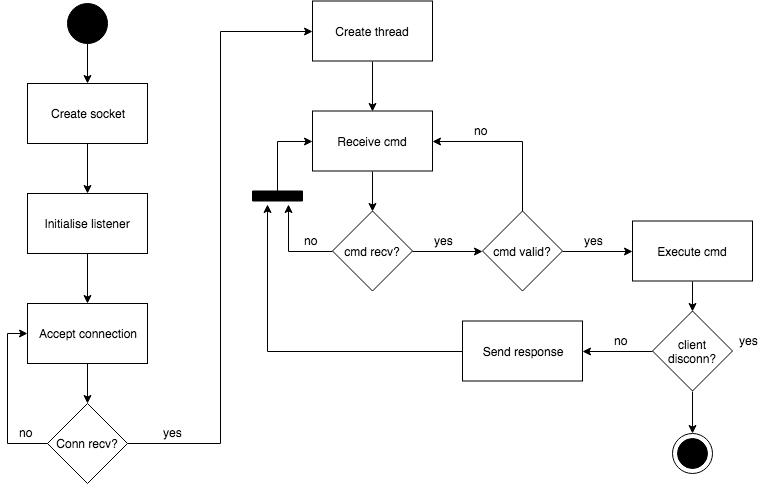
\includegraphics[width=0.8\textwidth]{Server.png}
	\caption{Flow chart depicting the process of server handling connections and client requests}
	\raggedright
	\label{fig:server}	
\end{figure}

\newpage
\section{Client Algorithms}

\begin{figure}[h]
	\centering
	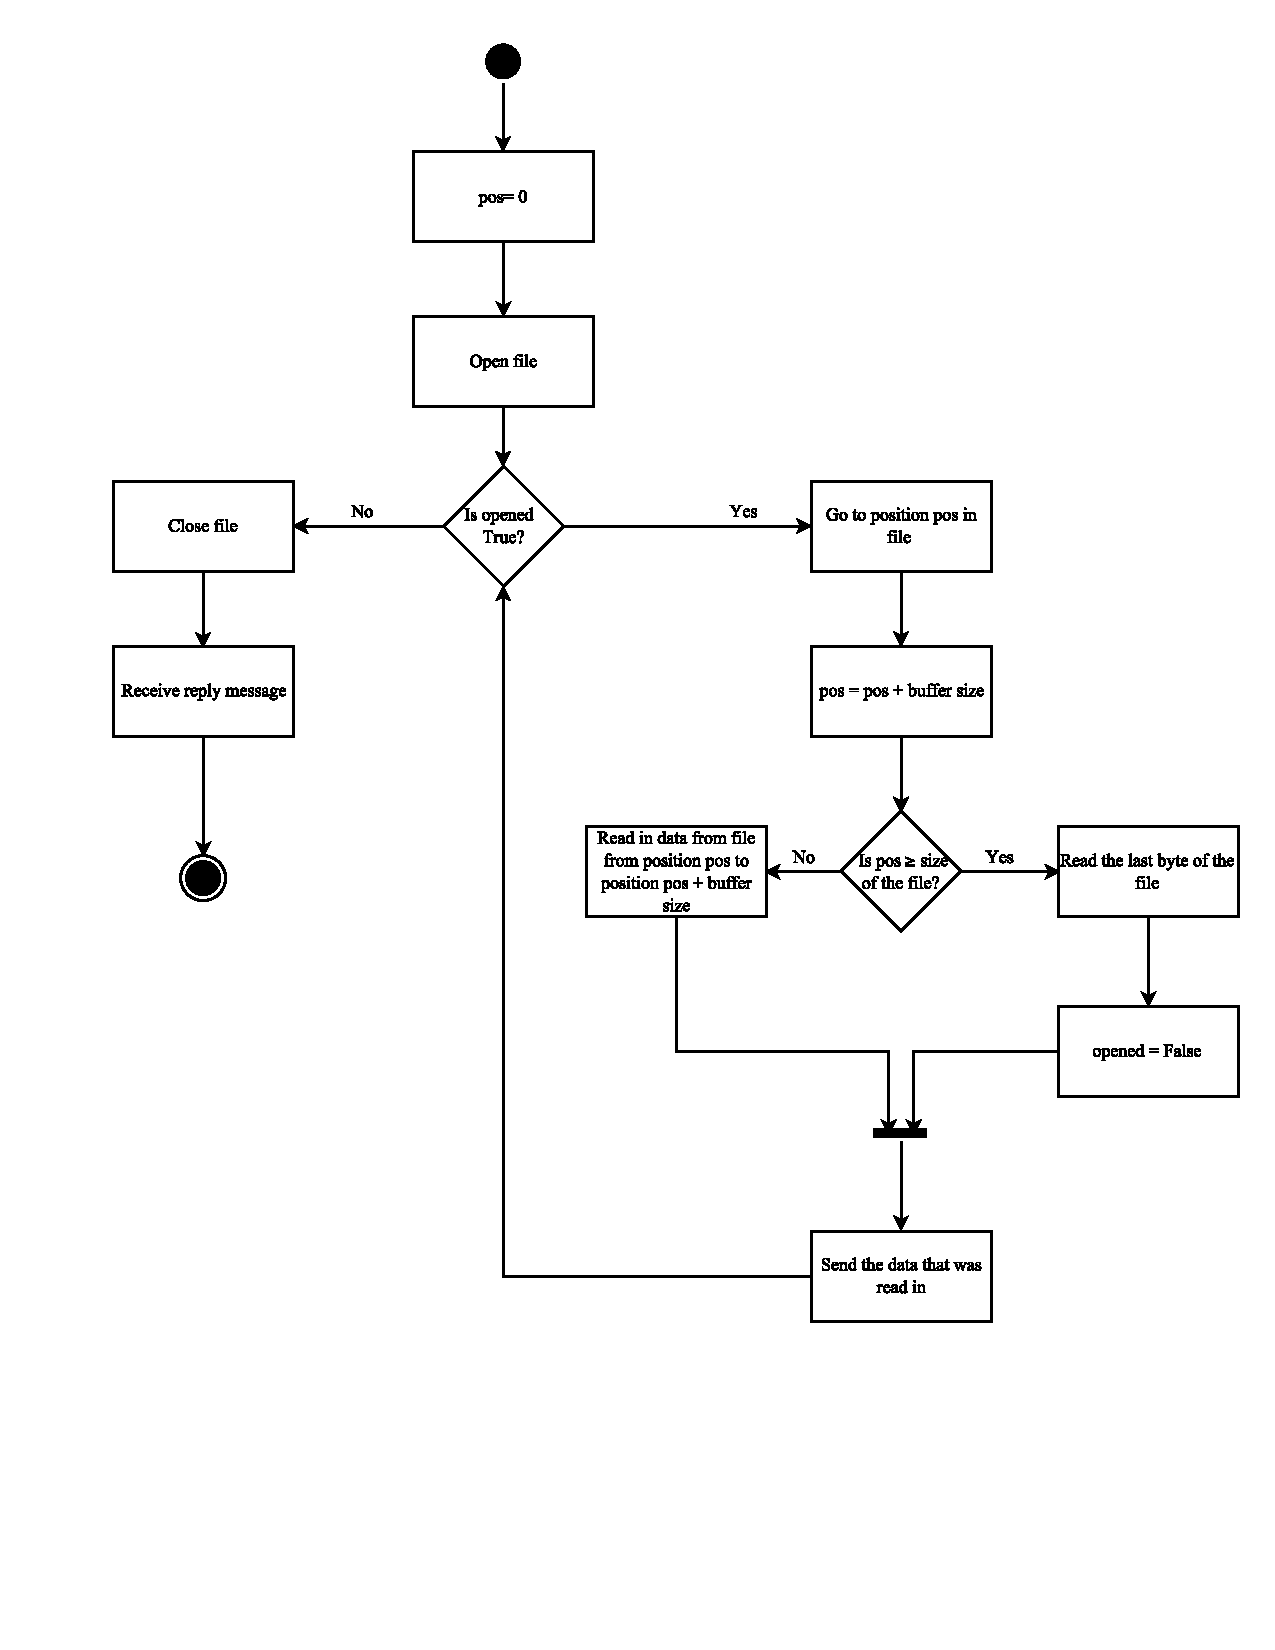
\includegraphics[width=0.6\textwidth]{uploadfile.pdf}
	\caption{Flow chart depicting the process of uploading a file to the server}
	\raggedright
	\label{fig:upload}	
\end{figure}

\end{appendix}

\end{document}

" vim: ts=4
" vim: tw=78
" vim: autoindent
" vim: shiftwidth=4